% CVPR 2022 Paper Template
% based on the CVPR template provided by Ming-Ming Cheng (https://github.com/MCG-NKU/CVPR_Template)
% modified and extended by Stefan Roth (stefan.roth@NOSPAMtu-darmstadt.de)

\documentclass[10pt,twocolumn,letterpaper]{article}

%%%%%%%%% PAPER TYPE  - PLEASE UPDATE FOR FINAL VERSION
\usepackage{cvpr}      % To produce the REVIEW version
%\usepackage{cvpr}              % To produce the CAMERA-READY version
%\usepackage[pagenumbers]{cvpr} % To force page numbers, e.g. for an arXiv version

% Include other packages here, before hyperref.
\usepackage{graphicx}
\usepackage{amsmath}
\usepackage{amssymb}
\usepackage{booktabs}


% It is strongly recommended to use hyperref, especially for the review version.
% hyperref with option pagebackref eases the reviewers' job.
% Please disable hyperref *only* if you encounter grave issues, e.g. with the
% file validation for the camera-ready version.
%
% If you comment hyperref and then uncomment it, you should delete
% ReviewTempalte.aux before re-running LaTeX.
% (Or just hit 'q' on the first LaTeX run, let it finish, and you
%  should be clear).
\usepackage[pagebackref,breaklinks,colorlinks]{hyperref}


% Support for easy cross-referencing
\usepackage[capitalize]{cleveref}
\crefname{section}{Sec.}{Secs.}
\Crefname{section}{Section}{Sections}
\Crefname{table}{Table}{Tables}
\crefname{table}{Tab.}{Tabs.}


%%%%%%%%% PAPER ID  - PLEASE UPDATE
\def\cvprPaperID{00000} % *** Enter the CVPR Paper ID here
\def\confName{CVPR}
\def\confYear{2023}

\begin{document}

%%%%%%%%% TITLE - PLEASE UPDATE
\title{Exploring the Use of Naive Bayes and kNN Classification for MNIST Data Set}

\author{Thomas Sigler\\
Georgia State University\\
Atlanta, Georgia\\
{\tt\small tsigler2@student.gsu.edu}
}
\maketitle

%%%%%%%%% ABSTRACT
\begin{abstract}
   The MNIST digit set presents the problem of classifying hand written digits by what number is represented. This can be done in a multitude of ways, and, in this paper, we'll explore using Naive Bayes and k-Nearest Neighbor (kNN). Naive Bayes utilizes conditional probability and prior information to inform estimation in generative classification. KNN utilizes a mutli-dimensional space of features with labels that outputs class membership of data. Both of these algorithms were utilized on the MNIST data set and became very good at classifying the digits correctly.
\end{abstract}

%%%%%%%%% BODY TEXT
\section{Introduction}
\label{sec:intro}

The MNIST data set is a compiled database of handwritten digits from students and census workers that is used to test machine learning models. Many machine learning models have been tested on the dataset and a nearly human comparable performance has been achieved using neural networks. Even with linear classifiers, the largest error rate observed has been 12\%. \cite{Alpher04}




% Update the cvpr.cls to do the following automatically.
% For this citation style, keep multiple citations in numerical (not
% chronological) order, so prefer \cite{Alpher03,Alpher02,Authors14} to
% \cite{Alpher02,Alpher03,Authors14}.


\begin{figure*}
  \centering
  \begin{subfigure}{0.7\linewidth}
    \fbox{\rule{0pt}{2in} \rule{.9\linewidth}{0pt}}
    \caption{Error rate over time of training.}
    \label{fig:short-a}
  \end{subfigure}
  \begin{subfigure}{0.25\linewidth}
    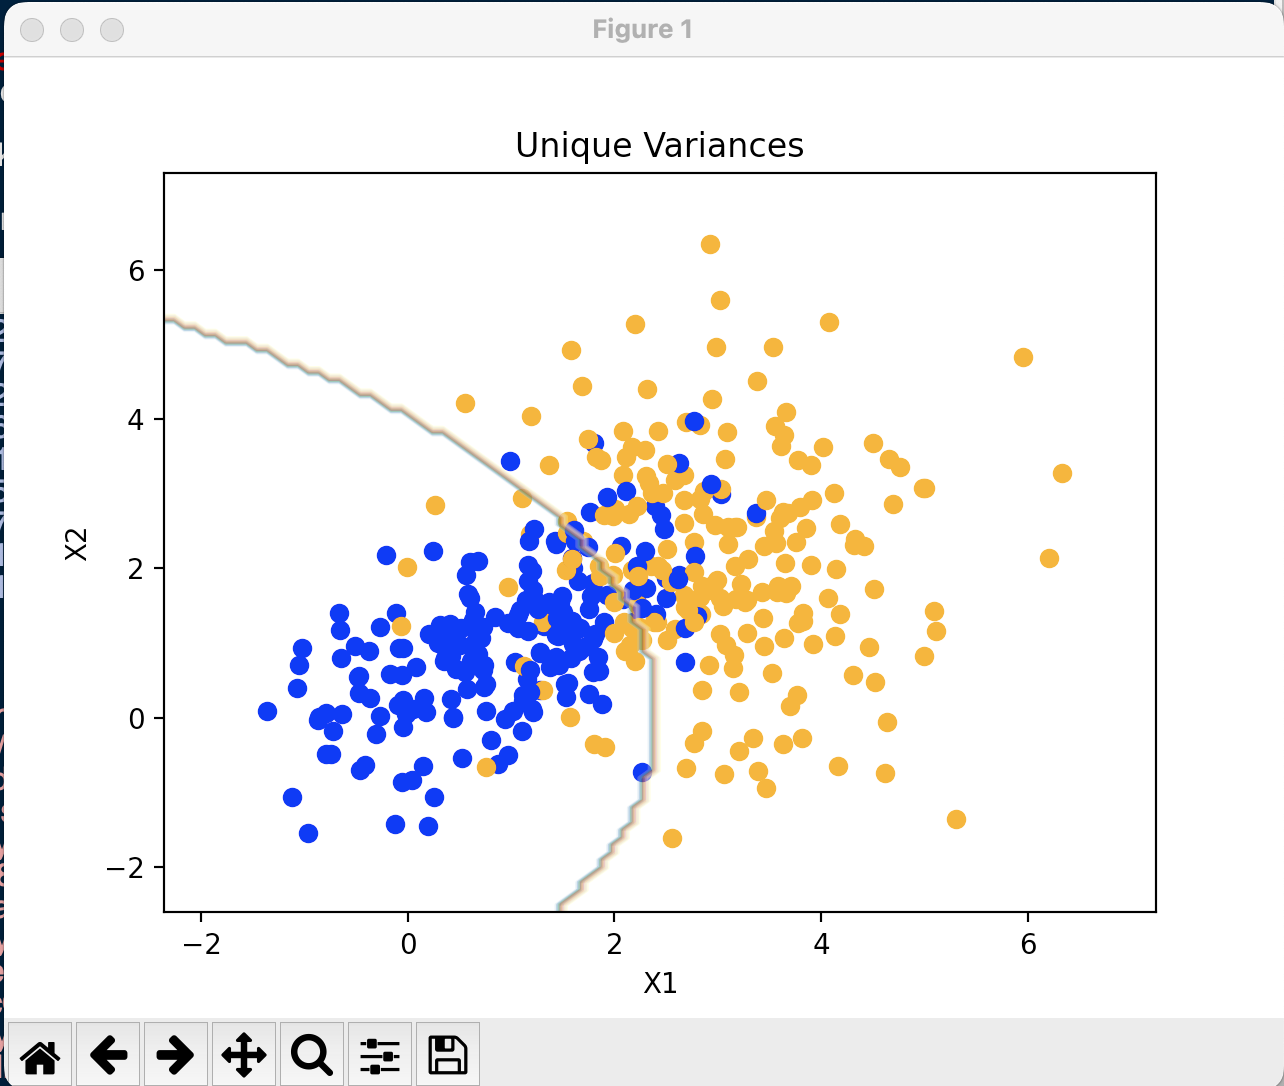
\includegraphics[scale=0.25]{images/Screenshot 2023-10-20 at 20.31.04.png}
    \caption{Most commonly misclassified images}
    \label{fig:short-b}
  \end{subfigure}
  \caption{The longer the algorithm was trained, the better attuned it was to classifying the images, but there remained images that were tricky for the algorithm to classify.}
  \label{fig:short}
\end{figure*}

%------------------------------------------------------------------------
\section{Models}
\label{sec:formatting}

The two methods that we use to classify the MNIST data set is Naive Bayes, using a Gaussian classification model and k-Nearest Neighbors (kNN). These two methods have a good track record of accurately, with small errors of classifying the MNIST data set.

\subsection{Naive Bayes Gaussian Classification}

Naive Bayes classification rest on the assumption that, given a classification, the features of that classification are linearly independent. Using this assumption, I applied the following equation:

\begin{equation}
    P(y=c|x_i)=\frac{P(x_i|y=c)P(y=c)}{P(x_i)}
\end{equation}

This forms the core of the Naive Bayes classifier, but using a Gaussian Model makes the equation more complex, supplying:

\begin{equation}
    P(X_i|y=c)=N(\mu_{ic},\sigma_{ic})=\frac{1}{\sqrt{2\pi\sigma_{ic}^2}}e^{-\frac{(x_i-\mu_{ic})^2}{2\sigma_{ic}^2}}
\end{equation}

From here, deriving the parameters of the equation yielded:

\begin{equation}
    \mu_{ic}=\frac{{\sum_{l=1}^m||\{y^{(l)}=c}\}x_i^{(l)}}{\sum_{l=1}^m||\{y^{(l)}=c\}}
\end{equation}

\begin{equation}
    \sigma_{ic}^2=\frac{\sum_{l=1}^m||\{y^{(l)}=c\}(x_{ic}^{(l)}-\mu_{ic})^2}{\sum_{l=1}^m||\{y^{(l)}=c\}}
\end{equation}

I also took into account prior probability P(Y):

\begin{equation}
    \hat{P}(y=c)=\frac{\sum_{i=1}^m||\{y^{(i)}=c\}}{m}=\hat{\pi}_c
\end{equation}

Finally, we arrived at the equation actually used for classification:

\begin{equation}
    \max_yP(y=c|x)=\log(\hat{\pi}_c)+\sum_{i=1}^n-\log(\sigma_{ic})-\frac{(x_i-\mu_{ic})^2}{2\sigma_{ic}^2}
\end{equation}

\subsection{k-Nearest Neighbors Classification}

The k-Nearest Neighbors algorithm is a classification algorithm used for supervised learning. The output is class membership of an image and we achieve this by having the members of the data's "local neighborhood" vote on its classification and taking the result as the most likely classification.

\section{Experiments}

I took the MNIST digit data set and began by running these basic algorithms on the training data to ascertain the best parameters for classification that these algorithms could produce given the training and test data that the data set provides by default. Further experiments were undertaken in each model using different pieces of the data set.

\subsection{Naive Bayes}

The Naive Bayes classification algorithm, using a Gaussian model, produced a --\% error rate after -- minutes of training, achieving average results for using this algorithm that would be measured as a benchmark for the rest of the experiments.\cite{Alpher02}

\subsection{k-Nearest Neighbor}

As of the writing of this draft, I do not have any results for k-Nearest Neighbor classification since the I have not programmed the algorithm in Python yet.

\section{Results}

As of the writing of this paper, I do not have any results stemming from classification experiments. I plan to try limiting the training data and seeing the results of the limits on the viablity of the models as they are given sparser data. I also plan on utilizing cross-validation to see if that improves the algorithms ability to condition the parameters for classification.

\section{Conclusions}

Naive Bayes is a suitable algorithm for achieving acceptable results in handwritten digit classification, achieving a --\% error rate on its best run. Both of these methods of classification are good for supervised learning, where labels are readily available for the data. The MNIST digit data set is a good start to training a machine learning algorithm for computer vision. 

\begin{table}[]
    \centering
    \begin{tabular}{c|c}
        Naive Bayes & kNN \\
        \hline
        1 & 2 \\
        3 & 4
    \end{tabular}
    \caption{An example table: Here I will compare the reliability of each of the algorithms and other results}
    \label{tab:my_label}
\end{table}

%%%%%%%%% REFERENCES
\newpage
{\small
\bibliographystyle{ieee_fullname}
\bibliography{egbib}
}

\nocite{*}

\end{document}
